\chapter{Análisis Teórico}
Se analizó el comportamento del circuito a pequeñas señales.

\section{Circuito de Polarización}\label{sec:polarizacion}
Como primer paso se analizó la polarización del circuito, ambos en su forma de carga pasiva (figura \ref{fig:pol_pasivo}) y activa (figura \ref{fig:pol_activo}).

\begin{figure} [ht]
    \centering
    \begin{minipage}{0.48\textwidth}
        \centering
        \begin{circuitikz}
            \ctikzset{resistors/scale=0.5};
            \draw
            (7,6.5) node[vcc](Vcc){$V_{CC}$}
            (5.5,5) node[npn](Q1){$Q_1$}
            (7,4) node[npn](Q2){$Q_2$}
            (Q1.E) |- (Q2.B)
            (Q1.C) |- (Vcc) (Q2.C) |- (Vcc)
            (Q1.B) to[R=$R_B$] ++(0,1.5) --(Vcc)
            (Q2.E) to[R=$R_E$] ++(0,-1) node[ground]{}
            ;
        \end{circuitikz}
        \caption{Circuito de Polarización con Carga Pasiva}
        \label{fig:pol_pasivo}
    \end{minipage}\hfill
    \begin{minipage}{0.48\textwidth}
        \centering
        \begin{circuitikz}
            \ctikzset{resistors/scale=0.5};
            \draw
            (7,6.5) node[vcc](Vcc){$V_{CC}$}
            (5.5,5) node[npn](Q1){$Q_1$}
            (7,4) node[npn](Q2){$Q_2$}
            (Q1.E) |- (Q2.B)
            (Q1.C) |- (Vcc) (Q2.C) |- (Vcc)
            (Q1.B) to[R=$R_B$] ++(0,1.5) --(Vcc)
            (Q2.E) to[I, l=$I_{ref}$] ++(0,-1) node[ground]{}
            ;
        \end{circuitikz}
        \caption{Circuito de Polarización con Carga Activa}
        \label{fig:pol_activo}
    \end{minipage}
\end{figure}

\subsection{Carga Pasiva}
En el circuito con Carga Pasiva, se resolvió analizando las mallas de entrada de los transistores. En ambos circuitos, para tener una comparación justa, se escogieron valores de componentes de forma que el punto de polarización de los transistores sean iguales.

\begin{align*}
    & V_{CC}-I_{B1}R_{B}-V_{BEon1}-V_{BEon2}-I_{E2}R_{E}=0 \\
    \vspace{1mm}
    & I_{E2} = \left(1 + h_{FE1}\right)\left(1 + h_{FE2}\right) I_{B1} \\

\end{align*}

\begin{equation}
    \Rightarrow & I_{E2} = \frac{V_{CC}-V_{BEon1}-V_{BEon2}}{R_E+\frac{R_B}{\left(1 + h_{FE1}\right)\left(1 + h_{FE2}\right)}}
    \label{I_E}
\end{equation}

Considerando que la influencia de de $R_B$ será despreciable frente a la de $R_E$, y que ambos transistores tienen la misma $V_{BEon}$ se puede aproximar \eqref{eq:pol_I_E2}. Luego se pueden obtener las $I_{CQ}$ de cada transistor.

\begin{equation}
    I_{E2} \approx \frac{V_{CC}-2V_{BEon}}{R_E}
    \label{eq:pol_I_E2}
\end{equation}

\begin{align}
    I_{CQ2} &= \frac{h_{FE2}}{h_{FE2}+1}\cdot I_{E2} \label{eq:icq2} \\ 
    I_{CQ1} &= \frac{h_{FE1}}{h_{FE1}+1}\cdot \frac{1}{h_{FE2}+1}\cdot I_{E2} \label{eq:icq1}
\end{align}

Recorriendo las mallas de salida se obtuvieron las $V_{CEQ}$ de cada transistor.

\begin{align}
    V_{CEQ2} &= V_{CC} - I_{E2} R_E \\
    V_{CEQ1} &= V_{CC} - I_{E2} R_E - V_{BEon} 
\end{align}

\subsection{Carga Activa}

A partir de la ecuación de Sah \eqref{eq:sah} para cada uno de los transistores se puede encontrar la razón entre la corriente de salida y de referencia.
\begin{equation}
    I_D = K' \frac{W}{L}\cdot (V_{GS}-V_{TH})^2
    \label{eq:sah}
\end{equation}

Considerando que por la configuración la tensión $V_{GS}$ será la misma para ambos transistores, y aproximando que, dado que se utilizarán transistores del mismo modelo, se puede aproximar que 

\begin{equation}
    I_o = \frac{(W/L)_3}{(W/L)_4} \cdot I_{ref}
\end{equation}

Por otro lado, puede diseñarse la $I_{ref}$ recorriendo la malla de $Q_4$ y resolviendo $V_{GS}$ para la $I_D = I_{ref}$

\begin{equation}
    V_{GS} = V_{TH} + \sqrt{\frac{I_D}{K'}\cdot\frac{L}{W}}
\end{equation}

\begin{equation}
    I_{ref}=\frac{V_{DD}-V_{GS}}{R_{ref}}
    \label{eq:I_ref}
\end{equation}

Luego, los resultados de \eqref{eq:I_ref} pueden utilizarse en \eqref{eq:pol_I_E2}, \eqref{eq:icq2} y \eqref{eq:icq1}.

También a partir de la ecuación	 \eqref{eq:sah} se puede obtener las tensiones de polarización:

\begin{align}
    V_{DS} &= V_{CC} - I_B R_B - 2V_{BEon} \\
    V_{CEQ2} &= V_{CC} - V_{DS} \\
    V_{CEQ1} &= V_{CC} - V_{DS} - V_{BEon}
\end{align}

\section{Parámetros de Pequeña Señal}

Se estimaron los parámetros de pequeña señal de cada transistor de acuerdo al modelo de híbrido en la configuración de seguidor de emisor.

\begin{align}
    \hat{h_{fe}} &\approx \beta \\
    \hat{h_{ie}} &\approx \hat{r_\pi} = (\beta+1) V_T/I_{CQ} \\
    \hat{h_{oe}} &\approx \hat{r_{ce}}^{-1} = I_{CQ}/V_A
\end{align}

% Para simplificar el desarrollo se aproximó que $r_x \approx 0$ y $r_\mu \approx \infty$, de modo que el modelo del circuito incremental utilizado será el de la figura

A partir de estas expresiones, y utilizando los resultados de las polarizaciones obtenidas en la sección \ref{sec:polarizacion}, se obtuvieron los valores numéricos de los parámetros de los modelos de pequeña señal.

\begin{figure} [ht]
    \centering
    \begin{minipage}[b]{0.48\textwidth}
        \centering
        \begin{circuitikz}
            \ctikzset{resistors/scale=0.5, capacitors/scale=0.5};
            \draw (0,0) node[anchor = east](ei){$e$} to[short,o-o] ++(7,0) node[anchor=west](eo){$e$};
            \draw (0,2) node[anchor = east](b){$b$} to[short,o-] ++(1,0) to[R, l=$h_{ie}$,-*] ++(0,-2);
            \draw (1,2) to[short,*-] ++(1,0) to[C,l=$C_{eb}$,-*] ++(0,-2);
            \draw (7,2) node[anchor = west](c){$c$} to[short,o-] ++(-1,0) to[R, l=$1/h_{oe}$,-*] ++(0,-2);
            \draw (2,2) to[C,l=$C_{cb}$,*-*] ++(2,0);
            \draw (6,2) to[short,*-] ++(-2,0) to[cI,l=$h_{fe} i_b$,-*] ++(0,-2);
        \end{circuitikz}
        \caption{Modelo incremental en Emisor Común}
        \label{fig:inc_ec}
    \end{minipage}\hfill
    \begin{minipage}[b]{0.48\textwidth}
        \centering
        \begin{circuitikz}
            \ctikzset{resistors/scale=0.5, capacitors/scale=0.5};
            \draw (0,0) node[anchor = east](ci){$c$} to[short,o-o] ++(6,0) node[anchor=west](co){$c$};
            \draw (0,2) node[anchor = east](b){$b$} to[short,o-] ++(1,0) to[C, l=$C_{cb}$,-*] ++(0,-2);
            \draw (1,2) to[short,*-] ++(0,1) to[C,l=$C_{eb}$] ++(2,0) to[short,-*] ++(0,-1);
            \draw (6,2) node[anchor = west](e){$e$} to[short,o-] ++(-1,0) to[R, l=$1/h_{oe}$,-*] ++(0,-2);
            \draw (1,2) to[R,l=$h_{ie}$,*-*] ++(2,0);
            \draw (3,0) to[cI,l_=$h_{fe} i_b$,-*] ++(0,2) to[short,-*] ++(2,0);
        \end{circuitikz}
        \caption{Modelo incremental en Colector Común}
        \label{fig:inc_cc}
    \end{minipage}
\end{figure}

% Antes de analizar el modelo de pequeña señal del par Darlington en configuración de seguidor de emisor, es necesario encontrar los parámetros del modelo híbrido, dadas por las siguientes ecuaciones..
% Estaba Giacoletto, pero es mas facil las cuentas con hibrido. Nose si afecta el cambio
% Necesitamos trabajar con Giacoletto porque tenemos que ver las capacitancias parásitas para la alta frecuencia. Además se puede trabajar directamente con los resultados de las tablas.

% \begin{align}
%     hie = \frac{\beta V_T}{I_{C1}} \\
%     hfe = \approx \beta \\
%     \frac{1}{hoe_1} = \frac{V_{A}}{I_{CQ}} \\
% \end{align}
% De las cuales a partir de la polarizacion previamente calculada, se obtienen los siguientes valores.

% \begin{table}
%     \centering
%     \begin{tabular}{|c|c|c|}
%      & $Q_1$ & $Q_2$ \\
%     $hie$           &    &     \\
%     $hfe$           &    &      \\
%     $\frac{1}{hoe}$ &    &      \\
%     \end{tabular}
% \end{table}


%%  MEJORAR IMPEDANCIA DE SALIDA DE FUENTE DE CORRIENTE

% A su vez es necesario calcular la impedencia de salida de la fuente de corriente. Al ser esta la carga activa, su impedancia de salida es la que vera el par Darlington en reemplazo de la resistencia $R_E$.
% Ya que es aqui especificamente donde se ve la mejora al circuito basico, es primordial tener un valor numerico para resaltarla. Como se trata de una fuente espejo con MOS-FET, se estima la impedancia de salida con la expresion de la ecuacion \ref{eq:imp salida fte corriente}.
Dado que el espejo de corriente tiene como referencia una corriente continua, su influencia sobre el circuito incremental estará modelado como una impedancia, la cual será la impedancia de salida del espejo de corriente.

\begin{equation}
    R_O = \frac{V_A}{I_0} 
    \label{eq:imp salida fte corriente}
\end{equation}

\newpage
\section{Circuito Incremental}

Se analizó el circuito incremental a frecuencias medias. Para ello se utilizaron los modelos híbridos de pequeña señal (figura \ref{fig:inc_cc} con los capacitores en Circuito Abierto), en principio en el circuito de la figura \ref{fig:circuito_pasivo}. Como se mencionó en la sección anterior, para el caso del circuito con carga activa (figura \ref{fig:circuito_activo}), se aplicó el mismo circuito incremental, aunque en lugar de la resistencia $R_E$ se utilizó la impedancia de salida del espejo de corriente $R_O$.

% Se reemplazan los transistores bipolares por su modelo híbrido para la pequeña señal en las figuras \ref{fig:circuito_pasivo} y \ref{fig:circuito}. Para esta ultima se considera la impedancia de salida ($R_O$) de la fuente espejo, en vez de la resistencia $R_E$.
% Se llega de esta manera en el circuito incremental pertinente, ilustrado en la figura \ref{fig:circuito incremental darlington}.

% \begin{figure}[ht]
%     \centering
%     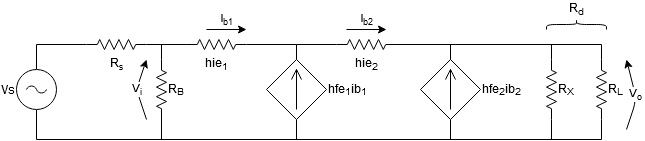
\includegraphics[scale=0.5]{2_teorico/figs/Incremental Darlington.png}
%     \caption{Circuito Incremental}
%     \label{fig:circuito incremental darlington}
% \end{figure}

\begin{figure}[ht]
    \centering
    \begin{circuitikz}
        \ctikzset{resistors/scale=0.5, capacitors/scale=0.5};
        \draw (0,0) to[sV,l=$v_s$] ++(0,2) to[R,l=$R_S$] ++(2,0) to[R,l=$R_B$, v=$v_i$] ++(0,-2) -- ++(-2,0);
        \draw (2,0) node[anchor = north]{} to[short,*-*] ++(4,0) node[anchor=north]{};
        \draw (6,2) to[R, l=$\frac{1}{h_{oe1}}$,*-*] ++(0,-2);
        \draw (2,2) to[R,l=$h_{ie1}$, f=$i_{b1}$,*-*] ++(2,0);
        \draw (4,0) to[cI,l_=$h_{fe1} i_{b1}$,-*] ++(0,2) to[short,-*] ++(2,0);
        \draw (6,0) node[anchor = north]{} to[short,*-*] ++(5,0) node[anchor=north]{};
        \draw (10,2) to[R, l=$\frac{1}{h_{oe2}}$,*-*] ++(0,-2);
        \draw (6,2) to[R,l=$h_{ie2}$, f=$i_{b2}$,*-*] ++(2,0);
        \draw (8,0) to[cI,l_=$h_{fe2} i_{b2}$,-*] ++(0,2) to[short,-*] ++(2,0);
        \draw (10,2) to[short,*-] ++(1,0) to[R,l=$R_E$] ++(0,-2) to[short,-*] ++(-1,0);
        \draw (11,2) to[short,*-] ++(1.5,0) to[R,l_=$R_L$, v^=$v_o$] ++(0,-2) to[short,-*] ++(-1.5,0);
    \end{circuitikz}
    \caption{Circuito incremental a frecuencias medias}
    \label{fig:incremental_MF}
\end{figure}

Para el cálculo de la impedancia de entrada y la ganancia de tensión, no se consideraron las resistencias de salida de los transistores. Estos sí fueron tomados en cuenta al calcular la impedancia de salida.

\subsection{Impedancia Entrada}

Conociendo las siguientes relaciones, aplicando pasaje a nivel de corriente se obtuvo la expresión para la impedancia de entrada $R_i$ del par Darlington.

\begin{align*}
    i_{b2} &= (1+h_{fe1}) i_{b1} \\
    \vspace{1mm}
    R_d &= R_E \parallel R_L
\end{align*}

\begin{equation}
    R_i = h_{ie1} + (1 + h_{fe1})\cdot h_{ie2} + (1 + h_{fe1})(1+h_{fe2})\cdot R_d
    \label{eq:R_i}
\end{equation}
\vspace{2mm}
Como se puede observar de la ecuación anterior, se espera una gran impedancia de entrada para nuestro componente activo,
del orden los cientos de $K\Omega$.
\vspace{2mm}

Por otro lado, la impedancia de entrada del amplificador estará dada por:
\begin{equation}
    R_{ia}=R_i \parallel R_B
    \label{R_ia}
\end{equation}
De la ecuación anterior se puede observar la importancia de $R_B$ en el circuito, ya que tomar un valor muy bajo 
me traería aparejada una gran pérdida en la impedancia de entrada de mi dispositivo. Sin embargo, también es 
necesario considerar que aumentar $R_B$ indiscriminadamente tiene un efecto colateral en la corriente de emisor 
de $Q_2$ dada por la ecuación[\ref{I_E}]. De esta manera, ya no podríamos asumir un error despreciable y la 
ecuación [\ref{pol_I_E2}] ya no sería válida. \par 
Por otro lado, la impedancia de entrada del sistema estará dada por:
\begin{equation}
    R_{is}=\frac{R_{ia}}{R_ia+R_s}
    \label{R_is}
\end{equation}
En un principio, se considerará a $R_s$ como la impedancia de un generador estándar de $50\Omega$. Luego, para medir 
$R_{ia}$ en la práctica se colocará una resistencia mayor.

\subsection{Ganancia de Tensión}
A partir de la ecuación \eqref{eq:R_i}, y observando las siguientes relaciónes, se obtuvo la ganancia de tensión $\Delta V$.

\begin{align*}
    v_o &= (h_{fe2}+1)\cdot i_{b2}\cdot R_d \\
    v_i &= i_{b1} \cdot R_i
\end{align*}

\begin{align}
    \Delta V &= \frac{v_o}{v_i} = \frac{v_o}{i_{b2}}\cdot \frac{i_{b2}}{i_{b1}}\cdot \frac{i_{b1}}{v_i} = (h_{fe2}+1)\cdot R_d \cdot (h_{fe1}+1)\cdot 1/ R_i \\
    \vspace{2mm}
    \Delta V &= \frac{R_d(1+h_{fe1})(1+h_{fe2})}{h_{ie1} + h_{ie2}(1+h_{fe2}) + R_d(1+h_{fe1})(1+h_{fe2})}
\end{align}

Sacando factor común se obtuvo que:

\begin{equation}
    \Delta V = \frac{1}{\frac{h_{ie1} + h_{ie2}(1+h_{fe2})}{R_d(1+h_{fe1})(1+h_{fe2})} + 1 }
    \label{eq:Av}
\end{equation}

Para poder considerar al circuito como seguidor de emisor($\Delta V \approx 1$), se debe cumplir que, observando la expresión \eqref{eq:Av}, se cumpla la relación

\begin{equation}
    R_d(1+h_{fe1})(1+h_{fe2}) >> h_{ie1} + h_{ie2}(1+h_{fe2})
\end{equation}

Por otro lado, la ganancia de tensión del sistema va a estar dada por:

\begin{equation}
    \Delta V_s = \frac{V_o}{V_s} = \frac{V_o}{V_i} \cdot \frac{V_i}{V_s} = \Delta V= \frac{R_{ia}}{R_{ia}+R_s}
\end{equation}

De la misma se desprende la importancia que tendrá $R_B$ como fue planteado en la sección anterior, intentando tomar valores 
tal que podamos mantener el comportamiento deseado.


\subsection{Ganancia de Corriente}

Se obtuvo que la ganancia de corriente estará dada por:

\begin{equation}
    \Delta i = (1+h_{fe1})(1+h_{fe2})
\end{equation}


Para la ganancia de corriente del sistema, se transformó la fuente de tensión por una fuente de corriente equivalente de valor $i_s=\frac{V_s}{R_s}$, 
donde se observó una relación de divisor de corriente entre $i_{b1}$ e $i_s$. 

\begin{equation*}
    i_{b1} = i_s\cdot \frac{R_S\parallel R_B}{R_i + R_S\parallel R_B}
\end{equation*}

Con esta relación se obtuvo finalmente la ganancia de corriente del sistema.


\begin{equation}
    \Delta_{is} = \Delta_i \cdot \frac{R_S\parallel R_B}{R_i + R_S\parallel R_B}
\end{equation}

\subsection{Impedancia de Salida}

Para el cálculo de la $r_o$ se realizó el procedimiento estándar de pasivar las fuentes independientes, 
colocar una señal de prueba a la salida y considerar nuevamente las resistencias $r_{ce}=1/h_{oe}$ de cada transistor.

\begin{figure}[ht]
    \centering
    \begin{circuitikz}
        \ctikzset{resistors/scale=0.5, capacitors/scale=0.5};
        \draw (2,0) to[short,*-] ++(-2,0) to[R,l=$R_S$] ++(0,2) to[short,-*] ++(2,0) to[R,l=$R_B$] ++(0,-2) -- ++(-2,0);
        \draw (2,0) node[anchor = north]{} to[short,*-*] ++(4,0) node[anchor=north]{};
        \draw (6,2) to[R, l=$r_{ce1}$,*-*] ++(0,-2);
        \draw (2,2) to[R,l=$h_{ie1}$, f=$i_{b1}$,*-*] ++(2,0);
        \draw (4,0) to[cI,l_=$h_{fe1} i_{b1}$,-*] ++(0,2) to[short,-*] ++(2,0);
        \draw (6,0) node[anchor = north]{} to[short,*-*] ++(4,0) node[anchor=north]{};
        \draw (10,2) to[R, l=$r_{ce2}$,*-*] ++(0,-2);
        \draw (6,2) to[R,l=$h_{ie2}$, f=$i_{b2}$,*-*] ++(2,0);
        \draw (8,0) to[cI,l_=$h_{fe2} i_{b2}$,-*] ++(0,2) to[short,-*] ++(2,0);
        \draw (10,2) to[short,*-] ++(1.5,0) to[sV,l^=$v_{op}$, i=$i_{op}$] ++(0,-2) to[short,-*] ++(-1.5,0);
        \draw (5,-0.5) node[anchor=north]{$r_{o1}'$} to[short] ++ (0,1) to[short] ++(-0.5,0) node[currarrow,xscale=-1]{};
        \draw (7,-0.5) node[anchor=north]{$r_{o1}$} to[short] ++ (0,1) to[short] ++(-0.5,0) node[currarrow,xscale=-1]{};
        \draw (9,-0.5) node[anchor=north]{$r_{o2}'$} to[short] ++ (0,1) to[short] ++(-0.5,0) node[currarrow,xscale=-1]{};
        \draw (11,-0.5) node[anchor=north]{$r_{o2}$} to[short] ++ (0,1) to[short] ++(-0.5,0) node[currarrow,xscale=-1]{};
    \end{circuitikz}
    \caption{Impedancias de salida}
    \label{fig:incremental_ro}
\end{figure}

Al tratarse de un acople de CC se sabe que el $r_o$ para dicha configuración está dado por:

\begin{align}
    r_{o1}'&= \frac{R_S\parallel R_B + h_{ie1}}{1 + h_{fe1}} \\
\end{align}

Consiguientemente, se llega a las siguientes expresiones donde se vuelve a aplicar la $r_o$ de un CC para el 
circuito equivalente:


\begin{align*}
    r_{o1} &= r_{o1}' \parallel r_{ce1} \\
    r_{o2}'&= \frac{r_{o1} + h_{ie2}}{1 + h_{fe2}}
\end{align*}

Obteniéndose finalmente la expresión para la $r_o$ de la configuración Darlington.

\begin{equation}
    r_o = r_{o2} = r_{o2}' \parallel r_{ce2}
\end{equation}

La impedancia de salida del sistema estará dada por:


\begin{equation}
    r_{oa} = r_{o} \parallel R_{E}
\end{equation}
    

\subsection{Respuesta en Frecuencia}
Utilizando el método de las constantes de tiempo, se estimaron las frecuencias de los polos de bajas y altas frecuencias. Como se observa más adelante, se pasivó el generador de la entrada y se calculó la constante de tiempo de cada circuito RC cuando solo uno de los capacitores se analiza.

\subsubsection{Bajas Frecuencias}
En el caso de las bajas frecuencias, las capacitancias de los transistores se pasivan como circuito abierto, y las capacitancias del circuito amplificador se pasivan como corto circuito.

\begin{figure}[ht]
    \centering
    \begin{circuitikz}
        \ctikzset{resistors/scale=0.5, capacitors/scale=0.5};
        \draw (0,0) to[R,l=$R_S$] ++(0,2) to[C,l=$C_S$] ++(2,0) to[R,l=$R_B$] ++(0,-2) -- ++(-2,0);
        \draw (2,0) node[anchor = north]{} to[short,*-*] ++(4,0) node[anchor=north]{};
        \draw (6,2) to[R, l=$\frac{1}{h_{oe1}}$,*-*] ++(0,-2);
        \draw (2,2) to[R,l=$h_{ie1}$, f=$i_{b1}$,*-*] ++(2,0);
        \draw (4,0) to[cI,l_=$h_{fe1} i_{b1}$,-*] ++(0,2) to[short,-*] ++(2,0);
        \draw (6,0) node[anchor = north]{} to[short,*-*] ++(5,0) node[anchor=north]{};
        \draw (10,2) to[R, l=$\frac{1}{h_{oe2}}$,*-*] ++(0,-2);
        \draw (6,2) to[R,l=$h_{ie2}$, f=$i_{b2}$,*-*] ++(2,0);
        \draw (8,0) to[cI,l_=$h_{fe2} i_{b2}$,-*] ++(0,2) to[short,-*] ++(2,0);
        \draw (10,2) to[short,*-] ++(1,0) to[R,l=$R_E$] ++(0,-2) to[short,-*] ++(-1,0);
        \draw (11,2) to[C,l=$C_L$, *-] ++(2,0) to[R,l_=$R_L$] ++(0,-2) to[short,-*] ++(-2,0);
        \draw (1,-0.5) node[anchor=north]{$r_{ia}$} to[short] ++ (0,1) to[short] ++(+0.5,0) node[currarrow]{};
        \draw (12,-0.5) node[anchor=north]{$r_{oa}$} to[short] ++ (0,1) to[short] ++(-0.5,0) node[currarrow,xscale=-1]{};
    \end{circuitikz}
    \caption{Circuito incremental a frecuencias bajas}
    \label{fig:incremental_LF}
\end{figure}

Como se observa en la figura \ref{fig:incremental_LF}, el capacitor $C_S$ ve una resistencia $R = R_S + r_{ia}$ con el capacitor $C_L$ pasivado. Además, el capacitor $C_L$ ve una resistencia $R = R_L + r_{oa}$ con el capacitor $C_S$ pasivado. De esta manera se pueden calcular las constantes de tiempo, y el polo de baja frecuencia se encontrará con la expresión \eqref{eq:fL}.

\begin{align*}
    \tau_1 &= C_S (R_S + r_{ia}) \\
    \tau_2 &= C_L (R_L + r_{oa})
\end{align*}

\begin{equation}
    f_L = \frac{1}{2\pi}\left(\frac{1}{\tau_1}+\frac{1}{\tau_2}\right)
    \label{eq:fL}
\end{equation}

Cabe notar que en el circuito de carga activa, el capacitor $C_L$ no está presente; por lo tanto, solo se conosideraron los efectos de solo el capacitor $C_S$ para su respuesta en frecuencia.

\subsubsection{Alta Frecuencia}
En el caso de las altas frecuencias, las capacitancias de los transistores fueron consideradas, y las del circuito externo amplificador fueron pasivadas como corto circuito.

Observando la figura \ref{fig:incremental_HF} se creyó que habría sido necesario aplicar el Teorema de Miller para calcular el efecto de las capacitancias $C_{eb}$. Sin embargo, si se da que en cada transistor se cumple que es un seguidor de emisor, es decir, que $\Delta_v \approx 1$, pueden despreciarse los efectos de estas capacitancias. Esto ocurre porque si ambos la base y el emisor tienen la misma tensión, no habrá flujo de corriente en esta capacitancia. De esta manera puede simplificarse y reacomodarse el circuito al de la figura \ref{fig:incremental_HFbis}.

\begin{figure}[ht]
    \centering
    \begin{circuitikz}
        \ctikzset{resistors/scale=0.5, capacitors/scale=0.5};
        \draw (0,0)  to[R,l=$R_S$] ++(0,2) to[short,-*] ++(1,0) to[R,l=$R_B$] ++(0,-2) -- ++(-1,0);
        \draw (1,0) node[anchor = north]{} to[short,*-*] ++(5,0) node[anchor=north]{};
        \draw (1,2) node[anchor = south]{} to[short,*-] ++(1,0) to[C, l=$C_{cb1}$,-*] ++(0,-2);
        \draw (2,2) to[short,*-] ++(0,1) to[C,l=$C_{eb1}$] ++(2,0) to[short,-*] ++(0,-1);
        \draw (6,2) to[R, l=$r_{ce1}$,*-*] ++(0,-2);
        \draw (2,2) to[R,l=$h_{ie1}$, f>_=$i_{b1}$,*-*] ++(2,0);
        \draw (4,0) to[cI,l_=$h_{fe1} i_{b1}$,-*] ++(0,2) to[short,-*] ++(2,0);
        \draw (6,0) node[anchor = north]{} to[short,*-*] ++(5,0) node[anchor=north]{};
        \draw (6,2) node[anchor = south]{} to[short,*-] ++(1,0) to[C, l=$C_{cb2}$,-*] ++(0,-2);
        \draw (7,2) to[short,*-] ++(0,1) to[C,l=$C_{eb2}$] ++(2,0) to[short,-*] ++(0,-1);
        \draw (11,2) to[R, l=$r_{ce2}$,*-*] ++(0,-2);
        \draw (7,2) to[R,l=$h_{ie2}$, f>_=$i_{b2}$,*-*] ++(2,0);
        \draw (9,0) to[cI,l_=$h_{fe2} i_{b2}$,-*] ++(0,2) to[short,-*] ++(2,0);
        \draw (11,2) to[short,*-] ++(1,0) to[R,l=$R_E$] ++(0,-2) to[short,-*] ++(-1,0);
        \draw (12,2) to[short,*-] ++(1.5,0) to[R,l_=$R_L$] ++(0,-2) to[short,-*] ++(-1.5,0);
    \end{circuitikz}
    \caption{Circuito incremental a frecuencias altas}
    \label{fig:incremental_HF}
\end{figure}

\begin{figure}[ht]
    \centering
    \begin{circuitikz}
        \ctikzset{resistors/scale=0.5, capacitors/scale=0.5};
        \draw (0,0)  to[C,l=$C_{cb1}$] ++(0,2) to[short,-*] ++(1,0) to[R,l=$R_S$] ++(0,-2) -- ++(-1,0);
        \draw (1,0) node[anchor = north]{} to[short,*-*] ++(5,0) node[anchor=north]{};
        \draw (1,2) node[anchor = south]{} to[short,*-] ++(1,0) to[R, l=$R_B$,-*] ++(0,-2);
        \draw (6,2) to[R, l=$r_{ce1}$,*-*] ++(0,-2);
        \draw (2,2) to[R,l=$h_{ie1}$, f=$i_{b1}$,*-*] ++(2,0);
        \draw (4,0) to[cI,l_=$h_{fe1} i_{b1}$,-*] ++(0,2) to[short,-*] ++(2,0);
        \draw (6,0) node[anchor = north]{} to[short,*-*] ++(5,0) node[anchor=north]{};
        \draw (6,2) node[anchor = south]{} to[short,*-] ++(1,0) to[C, l=$C_{cb2}$,-*] ++(0,-2);
        \draw (11,2) to[R, l=$r_{ce2}$,*-*] ++(0,-2);
        \draw (7,2) to[R,l=$h_{ie2}$, f=$i_{b2}$,*-*] ++(2,0);
        \draw (9,0) to[cI,l_=$h_{fe2} i_{b2}$,-*] ++(0,2) to[short,-*] ++(2,0);
        \draw (11,2) to[short,*-] ++(1,0) to[R,l=$R_E$] ++(0,-2) to[short,-*] ++(-1,0);
        \draw (12,2) to[short,*-] ++(1.5,0) to[R,l_=$R_L$] ++(0,-2) to[short,-*] ++(-1.5,0);
        \draw (1.5,-0.5) node[anchor=north]{$r_{ia}$} to[short] ++ (0,1) to[short] ++(0.25,0) node[currarrow]{};
        \draw (6.5,-0.5) node[anchor=north]{$r_{o1}$} to[short] ++ (0,1) to[short] ++(-0.25,0) node[currarrow,xscale=-1]{};
        \draw (7.5,-0.5) node[anchor=north]{$r_{i2}$} to[short] ++ (0,1) to[short] ++(0.25,0) node[currarrow]{};
    \end{circuitikz}
    \caption{Circuito incremental a frecuencias altas}
    \label{fig:incremental_HFbis}
\end{figure}

Con este esquema simplificado, se pudo calcular las constantes de tiempo, y obtener el polo de alta frecuencia con la expresión \eqref{eq:fH}.

\begin{align*}
    \tau_3 &= C_{cb1} (R_S \parallel r_{ia}) \\
    \tau_4 &= C_{cb2} (r_{o1} \parallel r_{i2})
\end{align*}

\begin{equation}
    f_H = \frac{1}{2\pi (\tau_3 +\tau_4)}
    \label{eq:fH}
\end{equation}

\section{Selección de Componentes}

\subsection{Limitaciones de la Plataforma de Medición} \label{sec:EE_limits}

Dado que el \textit{Electronics Explorer} sobre el cual se hicieron las mediciones tiene un límite de corriente de $1.5 \si{\ampere}$ en las salidas programables, se diseñaron los circuitos de forma de no saturar al dispositivo. La salida $V_{cc}$ no tiene limitación de corriente, pero la tensión es muy baja.

Como se planea utilizar un espejo de corriente, donde se consideró que ambos transistores n-mos son idénticos, las corrientes de polarización que se le pedirán a la fuente estarán dadas por:

\begin{equation*}
    I_{CQ} = \frac{h_{fe}}{h_{fe}+1} \cdot I_{EQ}; \quad I_{BQ} = \frac{1}{h_{fe}+1} \cdot I_{EQ}; \quad
    I_{CQ2} = I_o = I_{ref}; \quad I = I_{ref} + I_{CQ2} + I_{CQ1} + I_{BQ1}
\end{equation*}

\begin{equation}
    \Rightarrow I = I_{ref} \left(1 + \frac{h_{fe2}}{h_{fe2}+1} + \frac{1}{h_{fe2}+1}\cdot\frac{h_{fe1}}{h_{fe1}+1}+\frac{1}{h_{fe2}+1}\cdot\frac{1}{h_{fe1}+1}\right)
\end{equation}

Aproximando a valores altos de ganancias de corriente,

\begin{equation}
    I \approx I_{ref}\left(2+1/h_{fe2}\right)
\end{equation}

A partir de la expresión anterior se consideró entonces una cota máxima de la corriente de referencia:
\begin{equation}
    I_{ref} < 0.75 \si{\ampere}
    \label{eq:Iref}
\end{equation}

Finalmente, se puede confirmar que con los puntos de trabajo elegidos no habrían problemas con la plataforma de medición.

\subsection{Componentes Seleccionados y Parámetros Finales}

Tenieniendo en cuenta las limitaciones anteriores, primero se definieron los transistores a utilizar:

\begin{table}[ht]
    \centering
    \begin{tabular}{|r|l|l|l|r|r|l|l|r|r|l|}
    \cline{1-3} \cline{5-7} \cline{9-11}
    Transistor & Componente & Clase       &  & Comp.      & Valor & U                &  & Comp. & Valor & U                  \\ \cline{1-3} \cline{5-7} \cline{9-11} 
    $Q_1$      & BC547B     & BJT NPN     &  & $R_S$      & 50   & $\si{\ohm}$ &  & $R_L$      & 100   & $\si{\kilo\ohm}$   \\
    $Q_2$      & BC547B     & BJT NPN     &  & $R_B$      & 1.0   & $\si{\kilo\ohm}$ &  & $C_i$      & 100   & $\si{\nano\farad}$ \\
    $Q_3$      & BS170-D    & nMOS enr.  &  & $R_E$      & 900   & $\si{\ohm}$ &  & $C_L$      & 100   & $\si{\nano\farad}$ \\
    $Q_4$      & BS170-D    & nMOS enr. &  & $R_{ref}$  & 680   & $\si{\kilo\ohm}$ &  &           $V_{BEon}$& 0.6   &   $\si{\volt}$  \\ \cline{1-3} \cline{5-7} \cline{9-11} 
    \end{tabular}
    \caption{Componentes elegidos}
\end{table}

A partir de los valores de estos componentes, se calcularon los parámetros del circuito. Se consideraron como primera aproximación un valor de $V_T = 25.5 \si{\milli\volt}$ y $V_A = 60 \si{\volt}$. Dado que se esperan corrientes del orden de $\si{\micro\ampere}$ en $Q_1$, se tomó $h_FE = 150$. En $Q_2$ como se esperaban corrientes del orden de $10\si{\milli\ampere}$ se aproximó $h_FE = 290$.

\begin{table}
    \centering
    \begin{tabular}{|l|r|l|}
        \hline
        Característica  &   Valor   &   Unidad  \\
        \hline
        $V_{TH}$    &   $2.0$   &   $\si{\volt}$    \\
        $K'\frac{W}{L}$&$0.03$  &   $\si{\siemens/\volt}$ \\
        \hline
    \end{tabular}
    \caption{Características principales del BS170}
\end{table}

Para el caso de la carga activa, en lugar de utilizar $R_E = 900\si{\ohm}$ se utilizó $R_E' = 11.8 \si{\kilo\ohm}$.

\begin{table}[ht]
    \centering
    \begin{tabular}{|l|r|r|r|r|}
        \hline
        \multirow{2}{*}{} & \multicolumn{2}{c|}{Carga Pasiva} & \multicolumn{2}{c|}{Carga Activa} \\ \cline{2-5} 
         & $Q_1$ & $Q_2$ & $Q_1$ & $Q_2$ \\ \hline

        $I_{CQ} (\si{\ampere})$ & $29.6 \si{\micro}$& $8.64\si{\milli}$ & $29.6 \si{\micro}$& $8.64\si{\milli}$\\
        $V_{CE} (\si{\volt})$   & $0.60$            & $1.20$ & $0.60$ & $1.20$ \\
        $V_{CB} (\si{\volt})$   & $19.7 \si{\milli}$& $0.60$ & $19.7 \si{\milli}$& $0.60$\\ \hline

        $h_{fe} (\si{\ampere}/\si{\ampere})$ & $150$ & $290$ & $150$ & $290$ \\
        $h_{ie} (\si{\kilo\ohm})$ & $130$ & $0.977$ & $130$ & $0.977$ \\
        $h_{oe} (\si{\micro\siemens})$ & $0.493$ & $144$ & $0.493$ & $144$ \\
        $C_{cb} (\si{\pico\farad})$ & $3.2$ & $5.0$ & $3.2$ & $5.0$ \\ \hline

        $\Delta_{vi}$ & $0.9967$ & $0.9967$ & $0.9997$ & $0.9997$ \\
        $\Delta_{ii}$ & $151$ & $291$ & $151$ & $291$ \\
        $r_{ii} (\si{\mega\ohm})$ & $39.5$ & $0.260$ & $455$ & $3.01$ \\ 
        $r_{oi} (\si{\ohm})$ & $862$ & $5.91$ & $862$ & $5.91$ \\ \hline
    \end{tabular}
    \caption{Valores teóricos los transistores}
    \label{tab:vals_teo}
\end{table}

Para obtener el valor de $C_{cb}$ se remitió a la hoja de datos, dado que esta capacitancia es altamente sensible a la tensión entre la Base y el Colector.

Con estos resultados se verifica teóricamente que la aplicación adecuada de la carga activa no altera el punto de trabajo de los BJT.

\begin{table}[htt]
    \centering
    \begin{tabular}{|l|r|r|}
        \hline
         & \multicolumn{1}{c|}{Carga Pasiva} & \multicolumn{1}{c|}{Carga Activa} \\ \hline
        $\Delta_{v}$    & $0.9904$        & $0.9992$ \\
        $\Delta_{vs}$   & $0.9432$        & $0.9432$ \\ 
        $\Delta_{is}$   & $43.9\si{\kilo}$& $43.9\si{\kilo}$ \\ 
        $r_{i}(\si{\kilo\ohm})$ & $39.5$ & $455$ \\ 
        $r_{o}(\si{\ohm})$      & $5.91$ & $5.91$ \\
        $r_{ia}(\si{\kilo\ohm})$ & $1.00$ & $1.00$ \\ 
        $r_{oa}(\si{\ohm})$      & $5.87$ & $5.91$ \\
        $f_L(\si{\kilo\hertz})$  & $1.53$ & $1.53$  \\
        $f_H(\si{\mega\hertz})$  & $49.1$ & $48.9$  \\ \hline
    \end{tabular}
    \caption{Valores incrementales del circuito amplificador}
    \label{tab:vals_teo_sys}
\end{table}

\section{Comparacion Teórica Carga activa y pasiva}

A partir de los resultados observados en los cuadros \ref{tab:vals_teo} y \ref{tab:vals_teo_sys}, la aplicación de la carga activa por medio de un espejo de corriente trae mejoras al circuito sin cambiar su punto de polarización.

Al efectivamente aumentar la resistencia en la posición de $R_E$, aumenta la resistencia $R_d$, llevando a que la ganancia de tensión en cada transistor se acerque más a la unidad, mejorando el comportamiento de seguidor por emisor, y aumentando la impedancia de entrada del circuito.

%%Nose donde ponerlo, pero estimo que debe ir en esta seccion. Es mostrar como con la RO se obtiene mejor AV
%% Y la relacion de compromiso con RE(corriente y ganancia), lo que dijo en clase.